%!TEX root = ComputerScienceOne.tex

%%Chapter: Structs in C
\index{structures}
\index{encapsulation!C}

Strictly speaking, C is not an object-oriented programming language, 
it is an \emph{imperative} (or, relatedly a \emph{structured} or 
\emph{procedural}) programming language.  This means that C can be 
characterized as a language that changes a program's state through statements
and the use of function calls.  Though C does not have objects, it
does support a ``weak'' form of encapsulation through the use
of \emph{structures}.  Structures are a user-defined type that 
collects multiple pieces of data together into one logical unit.
Once defined, structures can be used in a program just like any
other variable type; structure variables can be declared, passed and returned
from functions, pointers to structures can be used, etc.
Structures form a ``weak'' form of encapsulation in that they only
provide the grouping of data.  The protection of data through 
visibility keywords is not supported.  The grouping of functions
that act on that data is also not readily supported.\footnote{You
\emph{can} define a structure with function pointers as elements, 
so structures could technically include ``methods'' but this is
not really what most people think of when considering object-oriented
paradigms.}  However, even this weak form provides a very useful
and convenient way to collect related pieces of \(  \)?ata.

\section{Defining Structures}
\index{structures!defining}

To define a structure, we use the keyword \mintinline{c}{struct}
along with the previously introduced keyword \mintinline{c}{typedef}.
To motivate an example, let's reconsider a student entity, which
has an ID (integer), first and last name (strings), and a GPA 
(a floating point number).  Each of these pieces of data can be
encapsulated into a structure as follows.

\begin{minted}{c}
typedef struct {
  int id;
  char *firstName;
  char *lastName;
  double gpa;
} Student;
\end{minted}

Note the syntax and naming conventions:
\begin{itemize}
  \item The elements of the structure (also referred to as components 
    or \emph{members}) are included inside curly brackets, 
  	delimited using semicolons (in contrast to an enumerated type which 
	is a list, these elements do \emph{not} constitute a list).
  \item A structure may contain any number of elements of any type.
  \item The name (identifier) of the structure is provided at the end, ended with
  	a semicolon.
  \item We use a modern naming convention: each element is named
  	using lower camel casing while the name of the structure itself
	uses upper camel casing.
\end{itemize}

In addition, structure declarations are generally placed in a header 
file along with any any function prototypes that use the structure as 
a parameter or a return type.  Once you have defined a structure you
can use it as you would a built-in variable type.  For example, 

\mintinline{c}{Student s;}

declares a \mintinline{c}{Student} structure with the variable
name \mintinline{c}{s}.

\subsection{Alternative Declarations}

In some examples and code bases you may find an alternative way
of declaring a structure that looks like the following.

\begin{minted}{c}
struct Student {
  ...
};
\end{minted}

This syntax omits the keyword \mintinline{c}{typedef} and places
the structure name at the beginning.  The difference is a bit 
technical (the original syntax creates an anonymous structure
with the \mintinline{c}{Student} identifier placed in the 
global namespace, while this declaration places the
\mintinline{c}{Student} identifier in the structure namespace), 
but one of the consequences of using this type of
declaration is that the \mintinline{c}{Student} identifier
is not in the global scope, so to declare a variable of the
type \mintinline{c}{Student} you need to further specify that
it is a structure using the following syntax.

\mintinline{c}{struct Student s;}

Further, you may also see another style, 

\begin{minted}{c}
typedef struct Student {
  ...
} Student;
\end{minted}

Which places the \mintinline{c}{Student} identifier in both
the global space \emph{and} in the ``structure'' space.  
Which style of declaration you use depends on several factors, 
but for simplicity we'll stick with the first style.

%One situation in which the second style is \emph{necessary} is 
%when the structure contains an instance of itself as a member
%(or a pointer to an instance of itself).  
%if the structure contains a pointer to a structure of the same type for
%example in a linked list implementation.
%This is not true; you just need to use the syntax \mintinline{struct Student *next} inside the structure.

In addition, you may see some older naming conventions use lowercase 
underscore naming for structure names.  In particular, \gls{posixLabel}
systems use names that end with \mintinline{c}{_t} (indicating
a structure \textbf{t}ype).  You should avoid such naming
conventions to avoid conflicts.

Finally, though C does not provide a mechanism for the protection of
data, many libraries and code bases will begin certain member variables
with underscore(s) to indicate that they are ``internal'' variables
used by the library and should \emph{not} be accessed or modified.
For example, \mintinline{c}{_someVariable} or \mintinline{c}{__anotherVariable} would indicate ``private'' variables that should
not be tampered with.  The C language itself would still allow you 
access and modify the variables, but doing so may violate assumptions
and expectations of the library code, leading to undefined behavior.

\subsection{Nested Structures}

Consider adding another member variable to the \mintinline{c}{Student}
structure to model a student's date of birth.  How might we model
a date?  Unix systems model time as a single integer value that
represents the number of milliseconds that have passed since the
Unix \emph{epoch}, January 1st, 1970 (also known as \gls{utcLabel}).  
For example, the New Horizons space probe
was launched on January 19th, 2006 at 19:00:00 UTC.  This corresponds
to 1,137,697,200, roughly 1.137 billion milliseconds since the
epoch.  Another way to model time is as a string.  There are several
standards for time representations, but the most common is \gls{isoLabel}
standard 8601 \cite{ISO:1988:IDE} which specifies time using a format that
includes a date, time and an offset from Greenwich Mean Time (GMT).
For example, the New Horizons launch date/time would be represented
as \mintinline{text}{"2006-01-19T19:00:00+00:00"}.

To keep things simple, we'll model our date using three numbers: a
year, a month and a date.  But how should we implement this?  
Conceptually, a date is a single entity, separating these three 
numbers doesn't make much sense.  This is a perfect opportunity to 
define another structure.

\begin{minted}{c}
typedef struct {
  int month;
  int day;
  int year;
} Date;
\end{minted}

Once we have defined a structure we can use it as we would a normal
variable, so it makes sense that we could include it in another structure.

\begin{listing}
\centering
\begin{minted}{c}
typedef struct {
  int id;
  char *firstName;
  char *lastName;
  double gpa;
  Date dateOfBirth;
} Student;
\end{minted}
\caption{A \mintinline{c}{Student} structure declaration}
\label{code:c:studentStructure}
\end{listing}

This is a good illustration of a form of \index{composition} 
\emph{composition} where 
one structure may be \emph{composed} of other structures.  Since
the \mintinline{c}{Student} structure ``owns'' an instance of the
\mintinline{c}{Date} structure, it is necessary to ensure that 
the \mintinline{c}{Date} structure is declared before the 
\mintinline{c}{Student} structure (just as we need to declare 
variables before we use them.

\section{Usage}

\subsection{Declaration \& Initialization}

Once we have defined a structure (and included the header file
it has been defined in), we can create instances using the usual
syntax.

\begin{minted}{c}
Student s;
Student t;
\end{minted}

These static declarations will allocate enough space on the stack
to hold all of the data associated with the structures (the two
\mintinline{c}{char *} pointers, \mintinline{c}{int}, and 
\mintinline{c}{double} and the three \mintinline{c}{int} variables
in the \mintinline{c}{Date} structure).  However, the values stored in 
each of the structure's member variables are undefined.  With
this style of declaration, C does not define default values.

Another way to declare instances of our structures
is to use the following syntax.

\begin{minted}{c}
Student s = {};
Student t = {
  12345678,
  "Grace",
  "Hopper",
  4.0,
  {
    12,
    9,
    1906
  }
};
\end{minted}

The first declaration creates a \mintinline{c}{Student} structure
with default values (zero for any numeric types, \mintinline{c}{null}
for any pointers).  The second creates a \mintinline{c}{Student}
structure initialized with the values provided in the curly brackets.
The order matters here and will match the ordering of the original
structure declaration.  Since the \mintinline{c}{dateOfBirth} is a
structure itself, a nested set of values within curly brackets is 
necessary.  One draw back to this type of declaration is that the
character pointers are statically declared.  The strings \mintinline{c}{"Grace"} and \mintinline{c}{"Hopper"} are initialized in a 
\emph{read-only} segment of memory, any attempts to change
the \emph{contents} of these strings are undefined behavior.  
The pointers themselves, however, can be reassigned.  The resulting
structure is visualized in Figure \ref{fig:studentStructViz}.

\begin{figure}
\centering
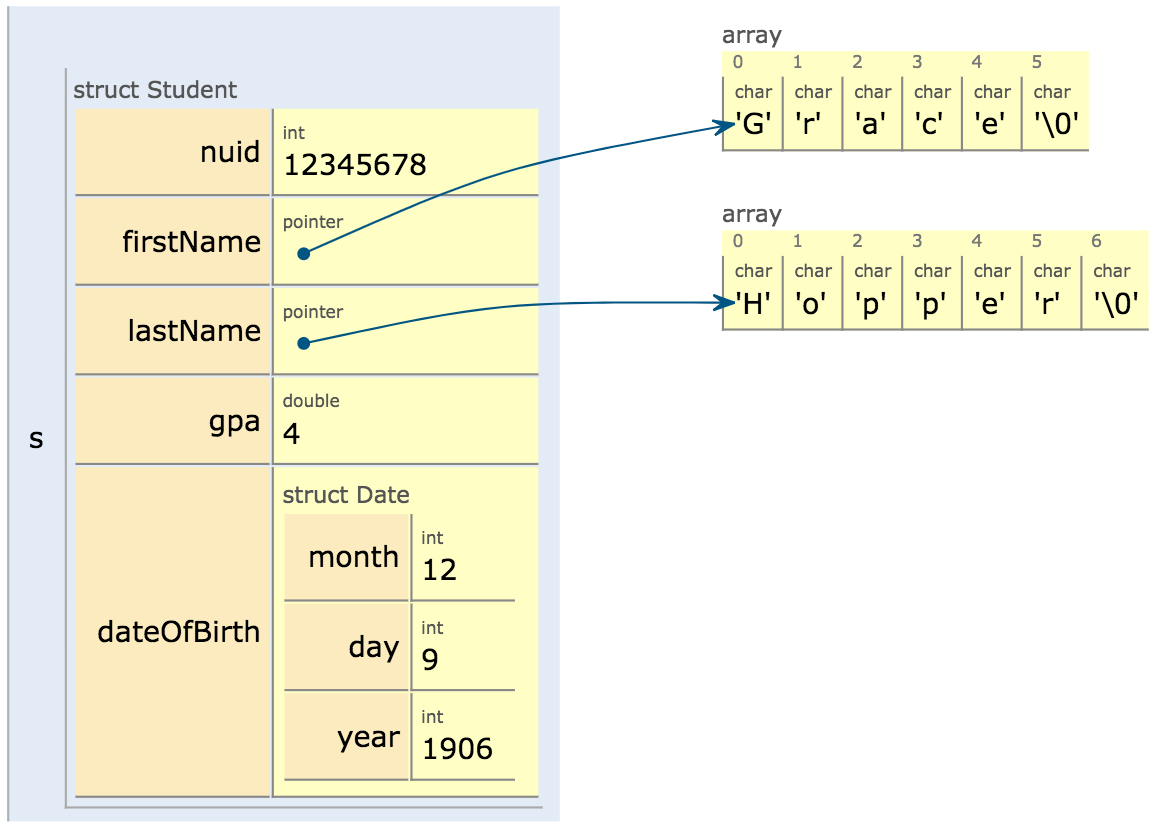
\includegraphics[scale=.25]{images/studentStructViz}
\caption{Visualization of an initialized \mintinline{c}{Student} structure.
Visualization generated by \url{http://pythontutor.com}}
\label{fig:studentStructViz}
\end{figure}

This static declaration allocates the structure on the stack.
Since structures consist of multiple pieces of data, their memory 
footprint is larger.  
Allocating larger and larger structures on the stack runs the
risk of running out of stack memory resulting in a 
\index{stack overflow} stack overflow.
To solve this, we can instead use dynamically allocated structures.

To dynamically allocate a structure, we use a pointer to a structure
and a call to \mintinline{c}{malloc()} to allocate enough space
for the structure.  Even though our structure is user-defined, we
can still use the \mintinline{c}{sizeof()} macro to determine
the number of bytes required by the structure.  The compiler and
macro are ``smart'' enough to look at the structure declaration and
determine the size of each of its variables and add up the total
number of bytes required.

\mintinline{c}{Student *s = (Student *) malloc(sizeof(Student) * 1);}

The multiplication by 1 in this example is not strictly necessary, but
emphasizes the fact that we are allocating space for one structure
and not an array of structures.  Initializing a dynamically allocated
structure like this does \emph{not} initialize any of its variables
as there are no default values defined by C.  Moreover, it does 
\emph{not} initialize memory for any pointer member variables.  For
example the \mintinline{c}{firstName} and \mintinline{c}{lastName}
pointers need to be manually initialized with additional 
\mintinline{c}{malloc()} calls.

\subsection{Selection Operators}

Once we have a declared structure, we need to access its member
variables and perhaps update them.  If we have a statically declared
structure, such as

\mintinline{c}{Student s;} 

we can use the \emph{direct component selector operator}, which is
simply just a period followed by the member variable we wish to 
access.  Commonly, this is referred to simply as the 
\index{dot operator} \emph{dot operator}.

\begin{minted}{c}
Student s;

//set values:
s.id = 87654321;
s.gpa = 3.9;

//access values:
printf("Name: %s, %s\n", s.lastName, s.firstName);
printf("GPA: %.2f\n", s.gpa);
\end{minted}

When structures are nested, we can use the dot operator multiple
times to access members variables of member variables.

\begin{minted}{c}
s.dateOfBirth.year = 2525;
s.dateOfBirth.month = 12;
s.dateOfBirth.date = 25;
\end{minted}

When we have a pointer to a structure, we cannot directly use
the dot operator.  Instead, we have to change the pointer into
a ``normal'' structure by dereferencing it, then we can use the
dot operator.  However, the dot operator has a higher order of
precedence than the dereferencing operator, thus parentheses are 
required:

\begin{minted}{c}
Student *s = ...;
(*s).id = 87654321;
\end{minted}

This can be a bit unwieldy, so C provides a convenience operator, 
the \emph{indirect component selector operator}, or more commonly,
the \index{arrow operator} \emph{arrow operator} that allows us 
to select a member variable
with a single operator that resembles a right-pointing arrow.

\begin{minted}{c}
Student *s = (Student *) malloc(sizeof(Student));

//set values:
s->id = 87654321;
s->gpa = 3.9;

//initialize the string variables:
s->firstName = (char *) malloc(sizeof(char) * 6);
strcpy(s->firstName, "Grace");
s->lastName = (char *) malloc(sizeof(char) * 7);
strcpy(s->lastName, "Hopper");

//access values:
printf("Name: %s, %s\n", s->lastName, s->firstName);
printf("GPA: %.2f\n", s->gpa);

s->dateOfBirth.year = 2525;
\end{minted}

Note the last line: the \mintinline{c}{dateOfBirth} member variable
was another structure, but not a pointer to a structure, so we
use the dot operator to access the \mintinline{c}{year} member
variable.  Alternatively, we could have defined \mintinline{c}{dateOfBirth}
to be a pointer, \mintinline{c}{Date *dateOfBirth;} in the 
\mintinline{c}{Student} structure.  If we had, then to access the 
\mintinline{c}{year} member variable using two arrow operators, 
\mintinline{c}{s->dateOfBirth->year}.

\section{Arrays of Structures}
\index{structures!arrays}

Just as we can create arrays of built-in types such as integers, 
we can also create arrays of our user-defined structures.  As
an example, the following creates an array of 10 \mintinline{c}{Student}
structures.  Once created, we can treat them like any other
array.  

\begin{minted}{c}
Student *roster = (Student *) malloc(sizeof(Student) * 10);

...

double sum = 0.0;
for(i=0; i<10; i++) {
  sum += roster[i].gpa;
}
double averageGpa = sum / 10;
\end{minted}

As in the example, we can index each element in the array, 
\mintinline{c}{roster}.  Once indexed, each element is a 
regular structure and so we use the dot operator to access
each of its member variables.  As with any other array, 
each element takes up a number of bytes, equal to 
\mintinline{c}{sizeof(Student)}.  We can swap and reassign
each element just like any other variable.  For example, 
the following code swaps the first two elements using
a temporary variable.

\begin{minted}{c}
Student temp = roster[0];
roster[0] = roster[1];
roster[1] = temp;
\end{minted}

Each of these operations copies over every byte that makes up
the structure.  For small structures, this isn't that big of
a deal.  However, for larger structures, this may become an
issue, especially if we do this often or pass structures around
to functions.

As an alternative, we could instead deal indirectly with structures
by creating an array of \emph{pointers} to structures.  Swapping
elements then involves only copying pointer values rather than
every byte that makes up the structure.  To do this, we use
the familiar pointer-to-pointer syntax.

\begin{minted}{c}
Student **roster = (Student **) malloc(sizeof(Student *) * 10);
for(i=0; i<10; i++) {
  roster[i] = (Student *) malloc(sizeof(Student) * 1);
}

//access each as pointers and use the arrow operator
roster[0]->id = 87654321;
roster[0]->gpa = 4.0;

//swap the first two *pointers*:
Student *temp = roster[0];
roster[0] = roster[1];
roster[1] = temp;
\end{minted}

As in the example above, if each element in the array is a pointer
to a structure, then we use the arrow operator to access each 
member variable.

The differences between these two approaches is illustrated in
Figures \ref{figure:arrayOfStructures} and \ref{figure:arrayOfStructurePointers}.
As presented, each \mintinline{c}{Student} structure takes 40 
bytes.\footnote{This is just an estimate and may vary on different systems
and compilers.  Usually, compilers use \emph{alignment} and may pad
structures with extra bytes in order to make it more efficient to store
in memory.}  With the first approach (as in Figure 
\ref{figure:arrayOfStructures}, each structure instance is stored 
contiguously in memory.  Swapping two records involves copying entire
blocks of 40 bytes.  In contrast, using pointers to structures as in
Figure \ref{figure:arrayOfStructurePointers} means that structures may
be stored non-contiguously in different memory locations.  Swapping
two structures is done indirectly by swapping pointers (only 8 bytes).
The difference in this particular example is not that great (8 vs.\ 40 bytes), 
but with larger structures it can become an issue.  Each approach has
its own advantages and disadvantages and one may be more appropriate 
than the other in different situations.

%\documentclass[12pt]{scrbook}
%
%\usepackage{tikz}
%\usepackage{minted}
%\usetikzlibrary{decorations.pathreplacing,arrows}
%
%\usepackage{fullpage}
%\usepackage{subfigure}
%\begin{document}
%
%
%Lorem Ipsum is simply dummy text of the printing and typesetting industry. Lorem Ipsum has been the industry's standard dummy text ever since the 1500s, when an unknown printer took a galley of type and scrambled it to make a type specimen book. It has survived not only five centuries, but also the leap into electronic typesetting, remaining essentially unchanged. It was popularised in the 1960s with the release of Letraset sheets containing Lorem Ipsum passages, and more recently with desktop publishing software like Aldus PageMaker including versions of Lorem Ipsum.
%
%xTODO: set vertical alignment of cells
%xTODO: curve the lines
%xTODO: lines should go to the top of the box

{\setmintedinline{bgcolor={}}

\begin{figure}
\centering

\begin{tikzpicture}[scale=0.75,transform shape]

% Define block styles
\tikzstyle{box} = [rectangle,
                   draw,
                   fill=white,
                   text width=3.0cm,
                   text height=0.9cm,
                   text centered,
                   inner sep=5pt,
                   node distance=1.85cm]

\tikzstyle{line} = [draw, -latex']; %

\draw[white] (-1, 0) rectangle (19, -1);
    \node [] (init) at (0,0) {\mintinline{c}{Student *roster}};

    \node [box, right of=init,node distance=5cm] (p0) {\mintinline{c}{roster[0]} \\
    (\mintinline{c}{Student})};
    %\node[node distance = 3cm,right of=p0] (d0) {?};
    %\draw[line] (p0) -- (d0);
    \node [box, below of=p0] (p1) {\mintinline{c}{roster[1]} \\
    (\mintinline{c}{Student})};
    %\node[node distance = 3cm,right of=p1] (d1) {?};
    %\draw[line] (p1) -- (d1);
    \node [box, below of=p1] (p2) {\mintinline{c}{roster[2]} \\
    (\mintinline{c}{Student})};
    %\node[node distance = 3cm,right of=p2] (d2) {?};
    %\draw[line] (p2) -- (d2);
    \node [below of=p2,node distance=2.0cm] (pd) {$\vdots$};
    \node [box, below of=pd,node distance=2.0cm] (pn) {\mintinline{c}{roster[n-1]} \\
    (\mintinline{c}{Student})};
    %\node[node distance = 3cm,right of=pn] (dn) {?};
    %\draw[line] (pn) -- (dn);
    \path [line] (init) -- (p0);
    
    \draw [decorate,decoration={brace,amplitude=6pt,mirror},xshift=4pt,yshift=0pt] (6.75, -0.8) -- (6.75, 0+0.9) node [align=left,black,midway,xshift=1.25cm]  {40 bytes};
    \draw [decorate,decoration={brace,amplitude=6pt,mirror},xshift=4pt,yshift=0pt] (6.75, -0.8-1.9) -- (6.75, 0+0.9-1.9) node [align=left,black,midway,xshift=1.25cm]  {40 bytes};
    \draw [decorate,decoration={brace,amplitude=6pt,mirror},xshift=4pt,yshift=0pt] (6.75, -0.8-1.9-1.9) -- (6.75, 0+0.9-1.9-1.9) node [align=left,black,midway,xshift=1.25cm]  {40 bytes};

    \draw [decorate,decoration={brace,amplitude=6pt,mirror},xshift=4pt,yshift=0pt] (6.75, -0.8-1.9-1.9-4) -- (6.75, 0+0.9-1.9-1.9-4) node [align=left,black,midway,xshift=1.25cm]  {40 bytes};


\end{tikzpicture}

\caption[Contiguous Structure Array]{An array of structures.  Each record is stored in a contiguous manner one after the other.}
\label{figure:arrayOfStructures}
\end{figure}
}

%\end{document}



{\setmintedinline{bgcolor={}}

\begin{figure}
\centering

\begin{tikzpicture}[scale=0.75,transform shape]

% Define block styles
\tikzstyle{box} = [rectangle,
                   draw,
                   fill=white,
                   text width=3.0cm,
                   %text height=0.9cm,
                   text centered,
                   inner sep=5pt,
                   node distance=1.25cm]

\tikzstyle{struct} = [rectangle,
                   draw,
                   fill=white,
                   text width=2.5cm,
                   minimum height=2.0cm,
                   text centered,
                   inner sep=5pt,
                   node distance=1.25cm]

\tikzstyle{line} = [draw, -latex']; %

\draw[white] (-1, 0) rectangle (19, -1);
    \node [] (init) at (0,0) {\mintinline{c}{Student **roster}};

    \node [box, right of=init,node distance=5cm] (p0) {\mintinline{c}{roster[0]} \\
    (\mintinline{c}{Student*})};
    %\node[node distance = 3cm,right of=p0] (d0) {?};
    %\draw[line] (p0) -- (d0);
    \node [box, below of=p0] (p1) {\mintinline{c}{roster[1]} \\
    (\mintinline{c}{Student*})};
    %\node[node distance = 3cm,right of=p1] (d1) {?};
    %\draw[line] (p1) -- (d1);
    \node [box, below of=p1] (p2) {\mintinline{c}{roster[2]} \\
    (\mintinline{c}{Student*})};
    %\node[node distance = 3cm,right of=p2] (d2) {?};
    %\draw[line] (p2) -- (d2);
    \node [below of=p2,node distance=1.5cm] (pd) {$\vdots$};
    \node [box, below of=pd,node distance=1.5cm] (pn) {\mintinline{c}{roster[n-1]} \\
    (\mintinline{c}{Student*})};
    %\node[node distance = 3cm,right of=pn] (dn) {?};
    %\draw[line] (pn) -- (dn);
    \path [line] (init) -- (p0);
    

    \node[struct] (a) at (11, 2) {\mintinline{c}{Student} \\(40 bytes)};
    %\draw[line] (p0.east) -- (a.west);
    
    \draw[line] (node cs:name=p0,angle=0)
      .. controls +(east:1cm) and +(-2,0) .. (a.155);

    \node[struct] (b) at (12, -1) {\mintinline{c}{Student} \\(40 bytes)};
    \draw[line] (node cs:name=p1,angle=0)
      .. controls +(east:3cm) and +(-1,0) .. (b.155);

    \node[struct] (c) at (10, -4) {\mintinline{c}{Student} \\(40 bytes)};
    \draw[line] (node cs:name=p2,angle=0)
      .. controls +(east:1cm) and +(-2,0) .. (c.155);


    \node[struct] (d) at (13, -7) {\mintinline{c}{Student} \\(40 bytes)};
    \draw[line] (node cs:name=pn,angle=0)
      .. controls +(east:4cm) and +(-2,0) .. (d.155);

\end{tikzpicture}

\caption[Array of Structure Pointers]{An array of structure pointers.  Each record is a pointer that refers to a structure which may be stored non-contiguously in completely different memory locations.}
\label{figure:arrayOfStructurePointers}
\end{figure}
}


\subsubsection{Hybrid Approach}

It is also possible to take a ``hybrid'' approach to storing structures
in arrays that stores them both contiguously, but also allows you to reference
them indirectly through a pointer array.  This is essentially what we did
in Section \ref{subsection:contiguous2DArrays} when we created a contiguous
2-dimensional array of integers.  We made a single call to \mintinline{c}{malloc}
and then had to setup the pointers to each ``row.''  To do this with 
structures, we can do something similar.  First, we declare and allocate 
a dynamic array as before.

\begin{minted}{c}
int n = 10;
Student *rosterData = (Student *) malloc(n * sizeof(Student));
\end{minted}

Then, we can declare an array of \mintinline{c}{Student} pointers as well.

\begin{minted}{c}
Student **roster = (Student **) malloc(n * sizeof(Student *));
\end{minted}

But now we need to make each \mintinline{c}{roster[i]} pointer point
to the $i$-th record in \mintinline{c}{rosterData}.  Each record, 
\mintinline{c}{rosterData[i]} is a regular structure, but we need 
a pointer to it.  In order to get a pointer, we use the referencing
operator, \mintinline{c}{&rosterData[i]} and make each pointer point
to it.

\begin{minted}{c}
for(i=0; i<n; i++) {
  roster[i] = &rosterData[i];
}
\end{minted}

This approach is illustrated in Figure \ref{figure:arrayOfStructuresHybrid}.
Now we can indirectly reference each record in \mintinline{c}{rosterData}
via a pointer in the \mintinline{c}{roster} array.  

\begin{minted}{c}
roster[0]->nuid = 12345678;
\end{minted}

If we wanted to ``swap''
two records, we simply swap their pointers instead of their data.  Indeed,
care must be taken not to swap the data in \mintinline{c}{rosterData} otherwise
the pointers would become invalid and out-of-synch with the data array.

%\documentclass[12pt]{scrbook}
%
%\usepackage{tikz}
%\usepackage{minted}
%\usetikzlibrary{decorations.pathreplacing,arrows}
%
%\usepackage{fullpage}
%\usepackage{subfigure}
%\begin{document}
%
%
%Lorem Ipsum is simply dummy text of the printing and typesetting industry. Lorem Ipsum has been the industry's standard dummy text ever since the 1500s, when an unknown printer took a galley of type and scrambled it to make a type specimen book. It has survived not only five centuries, but also the leap into electronic typesetting, remaining essentially unchanged. It was popularised in the 1960s with the release of Letraset sheets containing Lorem Ipsum passages, and more recently with desktop publishing software like Aldus PageMaker including versions of Lorem Ipsum.
%
%xTODO: set vertical alignment of cells
%xTODO: curve the lines
%xTODO: lines should go to the top of the box

{\setmintedinline{bgcolor={}}

\begin{figure}
\centering

\begin{tikzpicture}[scale=0.75,transform shape]

% Define block styles
\tikzstyle{box} = [rectangle,
                   draw,
                   fill=white,
                   text width=3.0cm,
                   text height=0.9cm,
                   text centered,
                   inner sep=5pt,
                   node distance=1.85cm]

\tikzstyle{pbox} = [rectangle,
                   draw,
                   fill=white,
                   text width=3.0cm,
                   text height=0.3cm,
                   text centered,
                   inner sep=5pt,
                   node distance=1.25cm]

\tikzstyle{line} = [draw, -latex']; %

    \node [] (init) at (0,-1) {\mintinline{c}{Student **roster}};

    \node [pbox,right of=init,node distance=5cm] (p0) {\mintinline{c}{roster[0]} \\
    (\mintinline{c}{Student*})};
    %\node[node distance = 3cm,right of=p0] (d0) {?};
    %\draw[line] (p0) -- (d0);
    \node [pbox, below of=p0] (p1) {\mintinline{c}{roster[1]} \\
    (\mintinline{c}{Student*})};
    %\node[node distance = 3cm,right of=p1] (d1) {?};
    %\draw[line] (p1) -- (d1);
    \node [pbox, below of=p1] (p2) {\mintinline{c}{roster[2]} \\
    (\mintinline{c}{Student*})};
    %\node[node distance = 3cm,right of=p2] (d2) {?};
    %\draw[line] (p2) -- (d2);
    \node [below of=p2,node distance=1.25cm] (pd) {$\vdots$};
    \node [pbox, below of=pd,node distance=1.5cm] (pn) {\mintinline{c}{roster[n-1]} \\
    (\mintinline{c}{Student*})};
    %\node[node distance = 3cm,right of=pn] (dn) {?};
    %\draw[line] (pn) -- (dn);
    \path [line] (init) -- (p0);
    

    \node [] (init) at (13,2) {\mintinline{c}{Student *rosterData}};

    \node [box, below of=init,node distance=2cm] (d0) {\mintinline{c}{roster[0]} \\
    (\mintinline{c}{Student})};
    %\node[node distance = 3cm,right of=p0] (d0) {?};
    %\draw[line] (p0) -- (d0);
    \node [box, below of=d0] (d1) {\mintinline{c}{roster[1]} \\
    (\mintinline{c}{Student})};
    %\node[node distance = 3cm,right of=p1] (d1) {?};
    %\draw[line] (p1) -- (d1);
    \node [box, below of=d1] (d2) {\mintinline{c}{roster[2]} \\
    (\mintinline{c}{Student})};
    %\node[node distance = 3cm,right of=p2] (d2) {?};
    %\draw[line] (p2) -- (d2);
    \node [below of=d2,node distance=2.0cm] (pdd) {$\vdots$};
    \node [box, below of=pdd,node distance=2.0cm] (dn) {\mintinline{c}{roster[n-1]} \\
    (\mintinline{c}{Student})};
    %\node[node distance = 3cm,right of=pn] (dn) {?};
    %\draw[line] (pn) -- (dn);
    \path [line] (init) -- (d0);
    
    \draw [decorate,decoration={brace,amplitude=6pt,mirror},xshift=4pt,yshift=0pt] (6.75+8, -0.8) -- (6.75+8, 0+0.9) node [align=left,black,midway,xshift=1.25cm]  {40 bytes};
    \draw [decorate,decoration={brace,amplitude=6pt,mirror},xshift=4pt,yshift=0pt] (6.75+8, -0.8-1.9) -- (6.75+8, 0+0.9-1.9) node [align=left,black,midway,xshift=1.25cm]  {40 bytes};
    \draw [decorate,decoration={brace,amplitude=6pt,mirror},xshift=4pt,yshift=0pt] (6.75+8, -0.8-1.9-1.9) -- (6.75+8, 0+0.9-1.9-1.9) node [align=left,black,midway,xshift=1.25cm]  {40 bytes};

    \draw [decorate,decoration={brace,amplitude=6pt,mirror},xshift=4pt,yshift=0pt] (6.75+8, -0.8-1.9-1.9-4) -- (6.75+8, 0+0.9-1.9-1.9-4) node [align=left,black,midway,xshift=1.25cm]  {40 bytes};

    \draw [decorate,decoration={brace,amplitude=6pt},xshift=4pt,yshift=0pt] 
      (6.75-3.75, -0.8-1.9-1.9-2.5+.25) -- (6.75-3.75, 0+0.9-1.9-1.9-2.5-.25) node [align=left,black,midway,xshift=-1.1cm]  {8 bytes};

%\draw[->] (p0.east) -- (d0.west);
%\draw[->] (p1.east) -- (d1.west);
%\draw[->] (p2.east) -- (d2.west);
%\draw[->] (pn.east) -- (dn.west);

\draw[line] (node cs:name=p0,angle=0)
      .. controls +(east:1cm) and +(-2,0) .. (d0.160);

\draw[line] (node cs:name=p1,angle=0)
      .. controls +(east:1cm) and +(-2,0) .. (d1.160);

\draw[line] (node cs:name=p2,angle=0)
      .. controls +(east:1cm) and +(-2,0) .. (d2.160);

\draw[line] (node cs:name=pn,angle=0)
      .. controls +(east:1cm) and +(-2,0) .. (dn.160);

\end{tikzpicture}

\caption[Hybrid Array of Structures]{Hybrid Array of Structures.  The \mintinline{c}{rosterData} is an array of contiguous structures.  The \mintinline{c}{roster} 
array is an array of pointers that refer to each record.  Accessing elements in
\mintinline{c}{rosterData} is done indirectly through a pointer in \mintinline{c}{roster}}
\label{figure:arrayOfStructuresHybrid}
\end{figure}
}




%\end{document}



\section{Using Structures With Functions}

As with built-in types, we can use structures as parameters to functions
as well as the return type of functions.  Consider the following
examples.

\begin{minted}{c}
void foo(Student s);
Student bar();
\end{minted}

In the first prototype, we would pass a \mintinline{c}{Student} structure
\emph{by value} to the function.  As we've already seen, this would
mean that every byte of the structure would be copied onto the stack.
For larger structures, we risk a stack overflow while for even smaller
structures this can be very inefficient.  Likewise, the second prototype
would return a structure.  When assigned to a variable, every byte is
copied.  A better solution is to use dynamically
allocated structures, passing them by reference to functions, and
returning pointers to dynamically allocated instances as return types.
For example, the functions above would be better implemented as follows.

\begin{minted}{c}
void foo(const Student *s);
Student * bar();
\end{minted}

In the first example, we've used the \mintinline{c}{const} keyword which
prevents any changes to the structure's values (we may omit this if
we need to design a function that changes its values).  We will now
consider several idiomatic examples of using structure with functions.

\subsection{Factory Functions}

Properly creating and initializing structure instances can be a
complex and tedious task.  However, it is likely that we will need
to repeat this operation over and over.  We can simplify our task
if we write a utility function that creates a structure instance for us.
We provide the function the values we want initialized to.  
Such functions are sometimes referred to as \emph{factory} functions
as they can be used to manufacture as many instances as we want
(in object-oriented programming languages, such methods are called
constructors).

We will need to take care that we make \index{deep copy} \emph{deep} copies of 
any dynamically allocated elements such as strings.  Shallow
copies \index{shallow copy} where references are shared may lead to unexpected 
behavior as changes to one string may affect multiple structures.

\begin{minted}{c}
/**
 * This function creates a new student structure with the
 * given values.
 */
Student * createStudent(const char *firstName, 
                        const char *lastName, 
                        int id, 
                        double gpa) {

  Student *s = NULL;
  s = (Student *) malloc(sizeof(Student) * 1);

  //make a deep copy of the strings
  s->firstName = (char *)malloc(sizeof(char)*(strlen(firstName)+1));
  strcpy(s->firstName, firstName);
  s->lastName = (char *)malloc(sizeof(char)*(strlen(lastName)+1));
  strcpy(s->lastName, lastName);

  s->id = id;
  s->gpa = gpa;

  return s;
}
\end{minted}

Another common operation is to create a copy of a given structure.
We will want to again ensure that everything is a \emph{deep}
copy so that the two structures are not sharing references.  We
can easily do this by reusing the functionality we just wrote in
the factory function.

\begin{minted}{c}
/**
 * This function creates a new, deep copy of a Student 
 * structure .
 */
Student * copyStudent(const Student *s) {
  return createStudent(s->firstName, s->lastName, s->id, s->gpa);
}
\end{minted}

\subsection{To String Functions}

Another common operation with structures is to output their data
as a human-readable string representation.  We could write
a function that output a structure's member variables to the standard
output using \mintinline{c}{printf()}.  However, it would more 
useful if we created a general function that returned a 
string representation of the structure.  That way, we could decide
what to do with the string: output it to the standard output,
to a file, etc.  Not all structure instances will require the same 
length string.
Some students for example may have long names, while others have
short.  We can handle this by first calculating the length of 
the string necessary for whatever formatting we've chosen.

\begin{minted}{c}
/**
 * Returns a string representation of the given 
 * Student structure.
 */
char * studentToString(const Student *s) {

  int n = strlen(s->firstName) + 
          strlen(s->lastName) + 
          8 + //id, assumed to always be at most 8 digits
          4 + //gpa, assumed to be 0.0 - 4.0
          19; //other formatting characters
          
  char *str = (char *) malloc(sizeof(char) * n);

  sprintf(str, "%s, %s, ID = %d (GPA = %.2f)", 
                s->lastName, s->firstName, s->id, s->gpa);

  return str;
}
\end{minted}

Here, we've utilized a variation on the familiar \mintinline{c}{printf()}
function, \mintinline{c}{sprintf()} which ``prints'' the result not
to the standard output or a file, but to a string, specified as
the first argument.  This function would end up returning a string 
similar to the following for our previous example: 
\mintinline{text}{"Hopper, Grace, ID = 87654321 (GPA = 3.90)"}

\subsection{Passing Arrays of Structures}

We often also have need to pass arrays of structures to functions.
As an example, consider passing an entire roster of students to 
a function in order to compute the average GPA.  If we have an
array of structures, we would have a function that looked something
like the following.

\begin{minted}{c}
/**
 * Computes the average GPA of the Student structures in
 * the given roster (which is of size n).
 */
double computeAverageGpa(const Student *roster, int n) {
  double sum = 0.0;
  int i;
  for(i=0; i<n; i++) {
    sum += roster[i].gpa;
  }
  return sum / n;
}
\end{minted}

When we pass in the array of structures, it is not passed by
value.  That is, the total number of bytes for each student is
\emph{not} copied onto the call stack.  Nevertheless, as we've
previously seen it is sometimes preferable to maintain an array
of pointers to structures.  If we had an array of pointers, we 
would have a function that looks something like the following.

\begin{minted}{c}
/**
 * Computes the average GPA of the Student structures in
 * the given roster (which is of size n).
 */
double computeAverageGpa(const Student **roster, int n) {
  double sum = 0.0;
  int i;
  for(i=0; i<n; i++) {
    sum += roster[i]->gpa;
  }
  return sum / n;
}
\end{minted}

The only difference here is in how we access the \mintinline{c}{gpa}
member variable using the arrow operator instead of the dot 
operator.





